\documentclass{article}
\usepackage{ctex}
\usepackage{graphicx}
\usepackage{amsmath}
\usepackage{indentfirst}
\usepackage{titlesec}
\usepackage{setspace}
\usepackage{subfigure}
\usepackage{caption}
\usepackage{float}
\usepackage{booktabs}
\usepackage{geometry}
\usepackage{multirow}
\geometry{left=1.2cm,right=1.2cm,top=2cm,bottom=2cm}
\title{\songti \zihao{2}\bfseries 拉曼光谱实验报告}
\titleformat*{\section}{\songti\zihao{4}\bfseries}
\titleformat*{\subsection}{\songti\zihao{5}\bfseries}
\renewcommand\thesection{\arabic{section}}
\author{王启骅 PB20020580}
\begin{document}
	\maketitle
	\section{实验数据与分析}
	 \begin{figure}[!h]
		\centering
		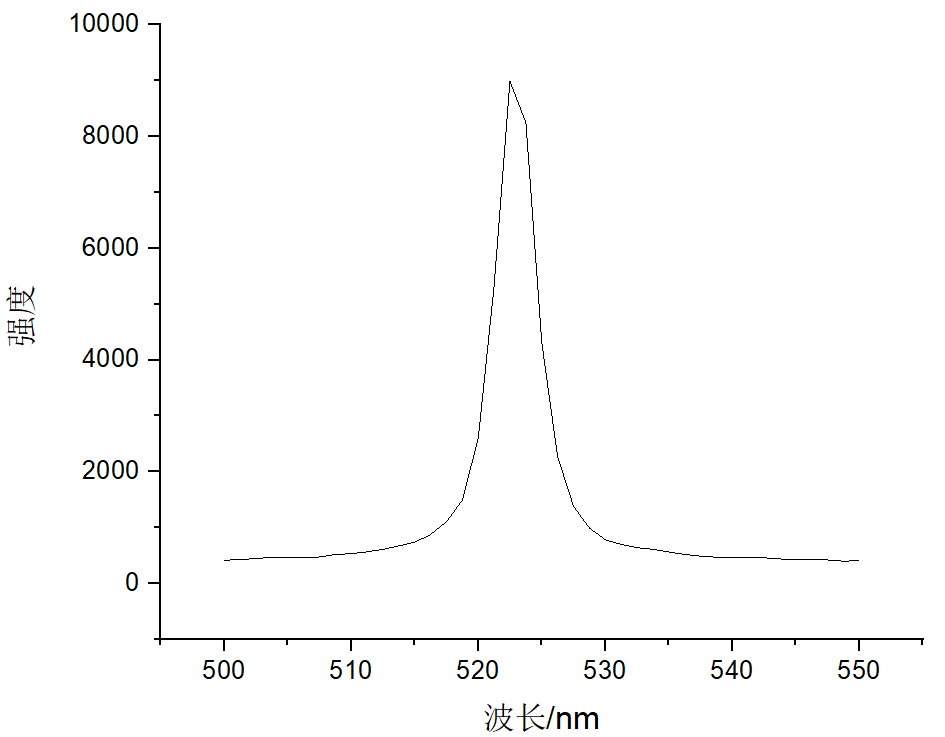
\includegraphics[scale=0.8]{Si}
		\captionsetup{font={small},labelfont=bf}
		\caption{\heiti\zihao{-5}Si拉曼光谱}
		
	\end{figure}

	 \begin{figure}[!h]
		\centering
		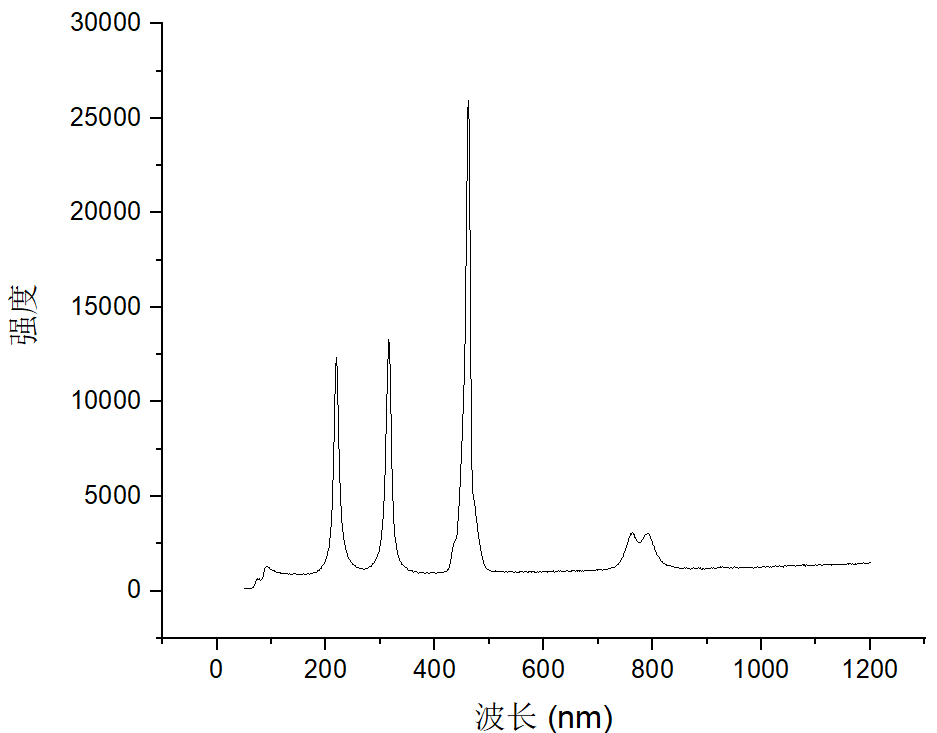
\includegraphics[scale=0.8]{CCl4}
		\captionsetup{font={small},labelfont=bf}
		\caption{\heiti\zihao{-5}CCl4拉曼光谱}
		
	\end{figure}


由图2可以看出,CCl4有3个拉曼峰,分别对应$ CCl_4 $的3种振动模式,分别为


1.四个Cl沿垂直于各自与C的连线的方向运动并保持重心不变。


2. C原子平行于正方形的一边运动,四个Cl原子同时平行于该边反向运动,分子重心保持不变。


3.两个Cl沿立方体一面的对角线作伸缩运动,另两个在对立面作位相的运动。
	
	
	\begin{figure}[!h]
		\centering
		\subfigure[未知样品1]{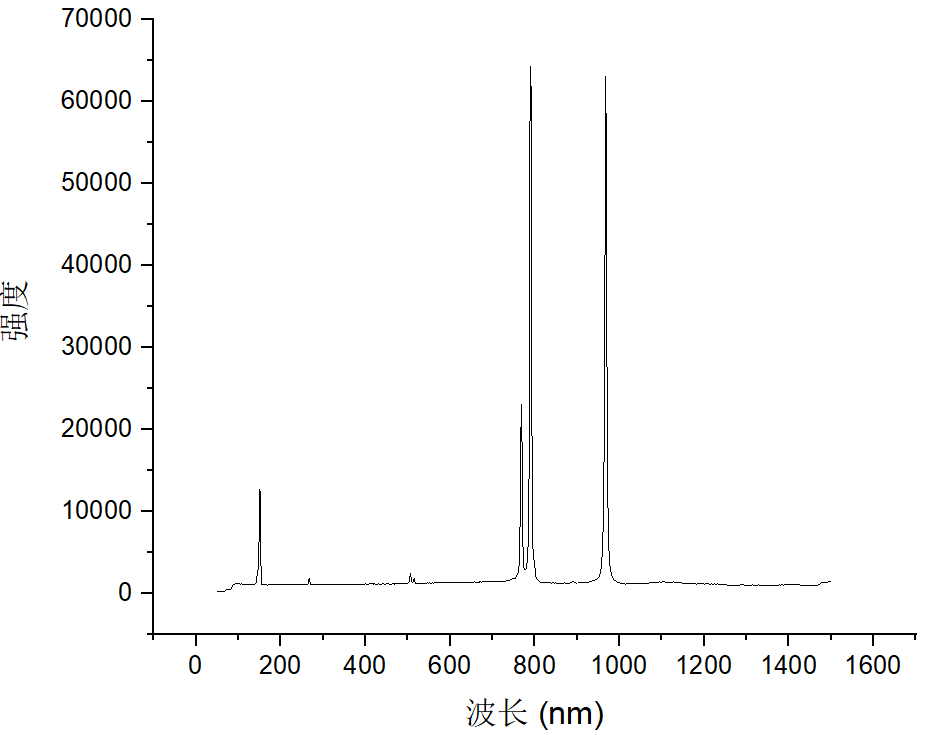
\includegraphics[scale=0.45]{CSi}}
		\subfigure[未知样品2]{	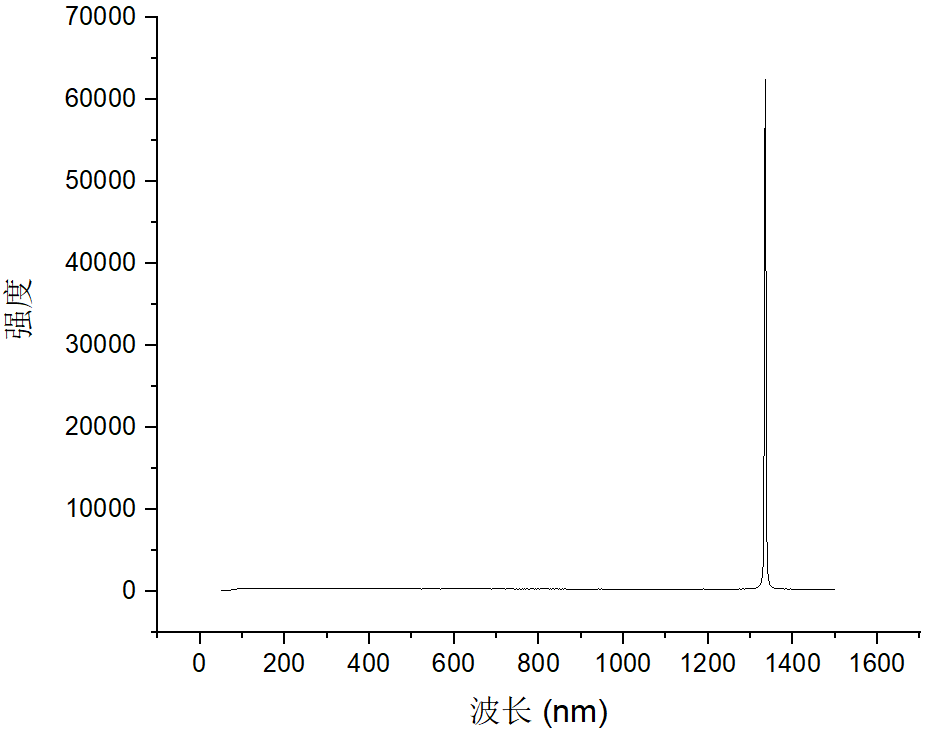
\includegraphics[scale=0.45]{C}}
		
		
		\captionsetup{font={small},labelfont=bf}
		\caption{\heiti\zihao{-5}未知样品拉曼光谱}
		
	\end{figure}


实验得到两个样品拉曼光谱如图3所示,根据查阅得到的谱图可以得到,未知样品1是碳化硅,未知样品2是金刚石。
\begin{figure}[!h]
	\centering
	\subfigure[碳化硅]{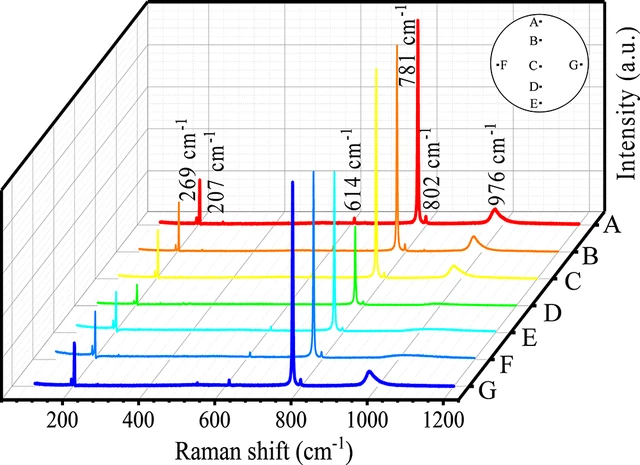
\includegraphics[scale=0.45]{碳化硅}}
	\subfigure[金刚石]{	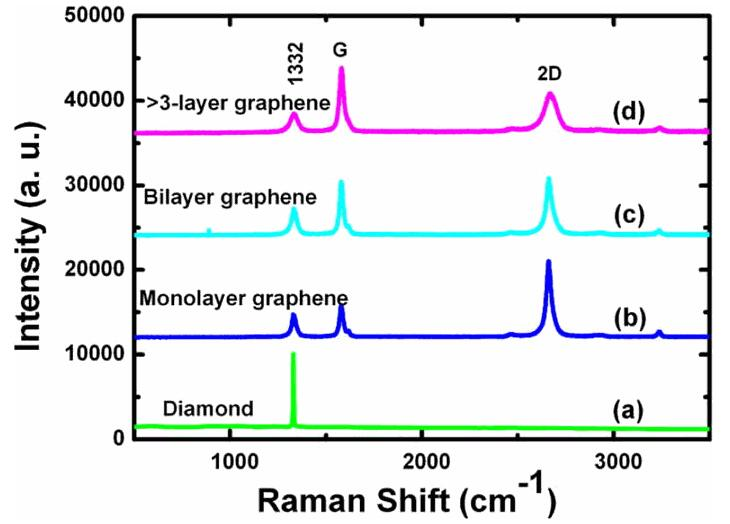
\includegraphics[scale=0.45]{金刚石}}
	
	
	\captionsetup{font={small},labelfont=bf}
	\caption{\heiti\zihao{-5}查阅得到拉曼光谱}
	
\end{figure}
	
	
	\section{思考题}
	1.由于反斯托克斯线频率较高,波长短,可以减小收集光的波长。
	
	
	2.激光功率,样品的浓度,以及测量软件中设置的参数(光谱采集时间等)。
	
	
	合适选择积分时间可以更好表示峰位特征。对焦的时候要尽可能让光聚焦在样品的剖面上,对于容器内溶液需要注意是否聚焦到样品内部,注意是否聚焦到样品正对光源的平面以收集较强的荧光信号。
	
	
	3.选择不同激发波长,Raman信号频移不变波长改变,荧光信号频移改变波长不变。如果是荧光信号,则该谱线应该有一定宽度,如果是杂散信号,则该谱线会非常尖细。可以通过增加积分时
	间来区分杂散信号,Raman峰和荧光峰⾼度随积分时间增加⽽上升,⽽杂散信号不会,且有些是随机产生,甚⾄
	会在重复测量后消失。


	4.金属原胞中只有1个原子,所以只有声学支没有光学支,不容易产生极化率的改变,
	Raman活性是根据极化率是否改变进行判断的,因而金属没有Raman活性。
	
	
	5.利用公式计算激光波数,
	\begin{equation}
		\frac{1}{\lambda}=\frac{1}{\lambda_0}-\Delta\frac{1}{\lambda}
	\end{equation}
	加入偏移后得到514.5nm下对应18103.35$cm^{-1}$,632.8nm下对应14469.78$cm^{-1}$.
\end{document}